% !TeX spellcheck = en_US
\documentclass[french]{yLectureNote}

\title{Outils Mathématiques}
\subtitle{Analyse dimensionnelle}
\author{Paulhenry Saux}
\date{\today}
\yLanguage{Français}

\professor{S.Deheuvels}%sebastien.deveuhels.irap.omp.eu

\usepackage{graphicx}%----pour mettre des images
\usepackage[utf8]{inputenc}%---encodage
\usepackage{geometry}%---pour modifier les tailles et mettre a4paper
%\usepackage{awesomebox}%---pour les boites d'exercices, de pbq et de croquis ---d\'esactiv\'e pour les TP de PC
\usepackage{tikz}%---pour deiffner + d\'ependance de chemfig
\usepackage{tkz-tab}
\usepackage{chemfig}%---pour deiffner formules chimiques
\usepackage{chemformula}%---pour les formules chimiques en \'equation : \ch{...}
\usepackage{tabularx}%---pour dimensionner automatiquement les tableaux avec variable X
\usepackage{awesomebox}%---Pour les boites info, danger et autres
\usepackage{menukeys}%---Pour deiffner les touches de Calculatrice
\usepackage{fancyhdr}%---pour les en-t\^ete personnalis\'ees
\usepackage{blindtext}%---pour les liens
\usepackage{hyperref}%---pour les liens (\`a mettre en dernier)
\usepackage{caption}%---pour la francisation de la l\'egende table vers Tableau
\usepackage{pifont}
\usepackage{array}%---pour les tableaux
\usepackage{lipsum}
\usepackage{yFlatTable}
\usepackage{multicol}
\newcommand{\Lim}[1]{\lim\limits_{\substack{#1}}\:}
\renewcommand{\vec}{\overrightarrow}
\newcommand{\norm}[1]{||\overrightarrow{#1}||}
\begin{document}
\setcounter{chapter}{4}
\chapter{Systèmes de coordonnées}
\section{Système cylindrique}
\begin{multicols}{2}

\subsection{Coordonnées}
Les coordonnées en fonctions de $z$ ne changent pas.
\subsubsection{Coordonnées cartésiennes en fonction des cylindriques}
\begin{itemize}
 \item $x = \rho \cos(\varphi)$
 \item $ y = \rho \sin(\varphi)$
\end{itemize}
\columnbreak

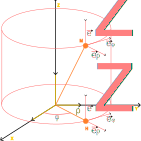
\includegraphics[scale=0.5]{base_c}

\end{multicols}
\subsubsection{Coordonnées cylindriques en fonction des cartésiennes}
\begin{itemize}
 \item $\rho = \sqrt{x^2+y^2}$
 \item $\varphi = \tan^{-1}(\frac{y}{x}) = \cos^{-1}(\frac{x}{\sqrt{x^2+y^2}})$\marginCritical{Attention aux conditions pour utiliser ces formules : celle avec $\tan^{-1}$ nécessite que y et x soient positifs et celle avec $\cos^{-1}$ que y soit positif.}
\end{itemize}

\subsection{Relation entre les vecteurs}
\begin{itemize}
 \item $\vec{e_{\rho}} = \cos( \varphi) \vec{e_x}+\sin( \varphi) \vec{e_y}$
 \item $\vec{e_{\varphi}} = -\sin( \varphi) \vec{e_x}+\cos( \varphi) \vec{e_y}$
\end{itemize}
\section{Système sphérique}
\subsection{Coordonnées}
\begin{multicols}{2}
\subsubsection{Lien avec les coordonnées cylindriques}
Dans les 2 cas, $\varphi$ ne change pas.
\begin{itemize}
 \item $\rho = r\sin\theta$
 \item $z = r\cos\theta$
\end{itemize}
\subsubsection{Coordonnées sphériques $\to$ cartésiennes}
\begin{itemize}
 \item $r = \sqrt{x^2+y^2+z^2}$
 \item $\theta = \cos^{-1}(\frac{z}{\sqrt{x^2+y^2+z^2}})$
 \item $\varphi = \tan^{-1}(\frac{y}{x}) = \cos^{-1}(\frac{x}{\sqrt{x^2+y^2}})$
\end{itemize}
\columnbreak

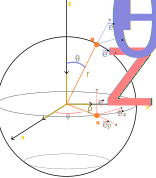
\includegraphics[scale=0.5]{base_s}
\end{multicols}


\subsubsection{Coordonnées cartésiennes $\to$ cylindrique}
\begin{itemize}
 \item $x = r\sin(\theta) \cos(\varphi)$
 \item $ y =  r\sin(\theta) \sin(\varphi)$
 \item $z = r\cos(\theta)$
\end{itemize}
\subsection{Relation entre les vecteurs}
\subsubsection{Base cylindrique}
\begin{itemize}
 \item $\vec{e_{\varphi}} = \vec{e_{\varphi}}$
 \item $\vec{e_{r}} = \sin(\theta) \vec{e_{\rho}} + \cos(\theta) \vec{e_z}$
 \item $\vec{e_{\theta}} = \cos(\theta) \vec{e_{\rho}} -\sin(\theta) \vec{e_z}$
\end{itemize}
\subsubsection{Base cartésienne}
\begin{itemize}
 \item $\vec{e_{\varphi}} = -\sin(\varphi)\vec{e_x} + \cos(\varphi)\vec{e_y}$
 \item $\vec{e_{r}} = \sin(\theta)\cos(\varphi) \vec{e_x} + \sin(\theta)\sin(\varphi) \vec{e_y}+\cos(\theta)\vec{e_z}$
 \item $\vec{e_{\theta}} = \cos(\theta)\cos(\varphi) \vec{e_x} +\cos(\theta)\sin(\varphi) \vec{e_y} - \sin(\theta)\vec{e_z}$
\end{itemize}
\end{document}

